\documentclass[10pt]{article}
\usepackage[letterpaper,margin=0.8in]{geometry}
\usepackage[T1]{fontenc}
\usepackage{lmodern}
\usepackage{microtype}
\usepackage{amsmath}
\usepackage{xcolor}
\usepackage{graphicx}
\usepackage{array,tabularx,booktabs}
\usepackage{enumitem}
\usepackage{caption}
\usepackage[hidelinks]{hyperref}

\setlength{\parindent}{0pt}
\setlength{\parskip}{4pt}
\setlist[itemize]{leftmargin=1.2em,topsep=2pt,itemsep=2pt,parsep=0pt}
\setlist[enumerate]{leftmargin=1.4em,topsep=2pt,itemsep=2pt,parsep=0pt}
\captionsetup{font=small,labelfont=bf,skip=4pt}

% Red placeholders: every one must be replaced with real facts before submission.
\newcommand{\fillin}[1]{\textcolor{red}{\textbf{[#1]}}}
\renewcommand{\topfraction}{0.9}
\renewcommand{\textfraction}{0.08}
\renewcommand{\floatpagefraction}{0.75}
\setcounter{topnumber}{3}
\setcounter{totalnumber}{5}
\newcolumntype{Y}{>{\raggedright\arraybackslash}X}

\title{\vspace{-1.2em}\textbf{Benchmark Cartography:\\Visually Auditing LLM Benchmark Answer Keys with Many-Model Agreement}}
\author{Arman Samayam (as21959@nyu.edu) \quad Padmapriya Venkatesh (px451@nyu.edu)\\
\small DS-GA 3001 Visualization for Machine Learning, Fall 2026 $\cdot$ Team 21}
\date{\vspace{-1em}}

\begin{document}
\maketitle

\begin{abstract}
\noindent LLM leaderboards rank models on benchmarks whose answer keys are partly wrong, but a reader
cannot see which questions are broken or whether they change the ranking. We adapt Dataset
Cartography from training epochs to models: we read all 14,042 MMLU questions through 150 public
models from the archived Open LLM Leaderboard and compute, for each question, how much
probability the models put on the official key, how much they disagree, and which alternative the
strongest models prefer. Against the 5,699 questions hand-checked by MMLU-Redux, low confidence
among the top 30 models finds wrong keys with AUPRC 0.355 (19$\times$ the 1.9\% base rate; 2PL IRT
reaches 0.211), and the top models' preferred alternative matches the human correction in 87\% of
cases where they agree. Removing the 106 known wrong keys swaps 28 of 11,175 model pairs, twice
what difficulty-matched random removals produce ($p=0.001$), yet no model enters or leaves the top
10. We built an interactive D3 tool that links a data map, a question inspector and a leaderboard
view, so an analyst can go from a suspicious region to a single question to its effect on rankings,
and evaluated it in think-aloud sessions with \fillin{n} LLM-evaluation practitioners.
Tool: \url{https://armansam17.github.io/Benchmark-Cartography/}.
\end{abstract}

\section{Introduction}

MMLU~\cite{mmlu} has about 14,000 four-option questions in 57 subjects and has been one of the most
reported LLM benchmarks. MMLU-Redux~\cite{redux} re-annotated 5,700 of them and found that 6.5\% have
a problem, including 1.9\% with a wrong answer key. Leaderboards separate neighbouring models by
fractions of a point (the median gap between adjacent models in our sample is 0.16 points of
accuracy), so a few hundred bad questions could in principle reorder them. Two practical questions
follow, and neither is answered by a table of scores: \emph{which} of the 8,343 questions nobody has
checked are likely broken, and does fixing them \emph{matter} for the ranking?

Dataset Cartography~\cite{cartography} answers the first kind of question for training data: it
tracks one model's probability on the gold label across training epochs, and mislabelled examples
fall in a ``hard-to-learn'' region of a confidence--variability map. An evaluation benchmark has no
training run, but a public leaderboard already holds hundreds of models' answers to every question.
We replace epochs with models.

\textbf{Problem statement.} Can the agreement and disagreement of many public LLMs, explored through
linked interactive views, help a person find likely broken MMLU questions, judge whether the key or
the models are wrong, and see how much those questions change the leaderboard?

\begin{itemize}
  \item \textbf{RQ1 (map).} Do MMLU-Redux-flagged questions fall in a distinct region of the data map?
  \item \textbf{RQ2 (detection).} How well do our scores rank flawed questions, compared with
    majority vote, low accuracy, 2PL IRT and random?
  \item \textbf{RQ3 (consequence).} Does removing or re-keying flawed questions reorder the
    leaderboard more than removing random questions of the same difficulty?
  \item \textbf{RQ4 (use).} What do LLM-evaluation experts discover with the tool, and how do they
    use its views to judge whether a flagged question is broken and whether it matters?
\end{itemize}

\textbf{Contributions.} (1) Cartography for an evaluation benchmark, with models in place of epochs
and a top-tier view that separates ``hard for most models'' from ``rejected by the strongest
models''. (2) Validation against human-verified errors, per error type, against an IRT baseline.
(3) An interactive tool that, to our knowledge, is the first to link question-level evidence to
leaderboard rankings against a difficulty-matched baseline. (4) A qualitative expert study of how
practitioners use that evidence.

\section{Related Work}

\textbf{Training dynamics and label errors.} Dataset Cartography~\cite{cartography} maps examples by
a model's confidence and variability across epochs; it needs training access, validates on
synthetic label noise, and its plots are static. Confident Learning~\cite{cl} estimates label errors
from one model's out-of-sample probabilities, and Northcutt et al.~\cite{pervasive} showed that
test-set label errors in ten classification benchmarks can change which model ranks first. Their
companion site, labelerrors.com, lists the errors but does not connect them to rankings.

\textbf{IRT for benchmarks.} Rodriguez et al.~\cite{rodriguez} and tinyBenchmarks~\cite{tiny} fit
item response theory to leaderboards; a 2PL model gives each question a difficulty and a
discrimination, and negative discrimination is a known sign of a miskeyed item. We use 2PL as our
main baseline and report where our scores overlap with it.

\textbf{MMLU quality.} MMLU-Redux~\cite{redux} hand-checked 5,700 MMLU questions in 57 subjects and
labelled each as fine or one of six error types, with a corrected answer for most wrong keys. It is
our ground truth for RQ1--RQ3.

\textbf{Interactive evaluation tools.} HELM~\cite{helm} publishes per-instance model outputs with a
results viewer; Zeno~\cite{zeno} lets analysts compare models on data slices; Calibrate~\cite{calibrate}
shows how interactive views expose problems in probabilistic output. None lets an analyst select
questions and see how removing or correcting them changes model rankings against a matched baseline,
which is the gap our leaderboard view fills.

\section{Data and Scores}

\textbf{Model outputs.} We sampled 150 models across 29 families from the archived Open LLM Leaderboard
details~\cite{openllm}, all evaluated with one harness version (lighteval \texttt{494ee122}, 5-shot),
so prompts are identical across models. For each model $m$ and question $q$ we take a softmax over the
log-likelihoods of options A--D, giving $p_m(q)$, the probability on the official key, and the model's
vote (its most likely option). The recovered key reproduces every model's recorded correctness
(0 conflicts in 2.1M checks). Models' macro accuracy (the mean of per-subject accuracy, as the
leaderboard reports it) ranges from 30.6\% to 80.2\%.

\textbf{Ground truth.} We joined MMLU-Redux 2.0 to MMLU by subject and normalised question and option
text, matching 5,699 of 5,700 questions (5,690 exactly). Of those, 5,329 are fine and 370 have an
error: 106 wrong keys, 132 unclear questions, 39 with multiple correct answers, 36 with no correct
answer, 25 with unclear options and 32 marked as needing an expert.

\textbf{Scores.} Following Dataset Cartography, and with the ``top tier'' being the 30 models (20\%)
with the highest macro accuracy:
\begin{itemize}
  \item \emph{confidence} and \emph{variability}: mean and standard deviation of $p_m(q)$ over models;
    \emph{correctness}: share of models whose vote is the key;
  \item \emph{top-tier confidence}: mean $p_m(q)$ over the top tier;
  \item \emph{ability alignment}: correlation across models between macro accuracy and $p_m(q)$
    (a healthy hard question is answered better by stronger models; a wrong key is the reverse);
  \item \emph{consensus alternative} and \emph{consensus share}: the non-key option most voted for by
    the top tier, and its share of their votes;
  \item \emph{vote entropy} (bits) over all models and over the top tier;
  \item \emph{2PL IRT}: $P(\text{correct}) = \sigma(a_q\theta_m - d_q)$, fitted by MAP with a
    zero-centred prior on the discrimination $a_q$ so that negative discrimination can appear. We use
    the intercept $d_q$ as difficulty, because the usual $b_q = d_q/a_q$ is unbounded as $a_q\to0$.
\end{itemize}
The cached tables, the model list, harness version, dataset revisions and SHA-256 checksums are in
\nolinkurl{data/processed/manifest.json}, and every number below is produced by scripts in the repository.

\section{The Tool}

\begin{figure}[!htb]
  \centering
  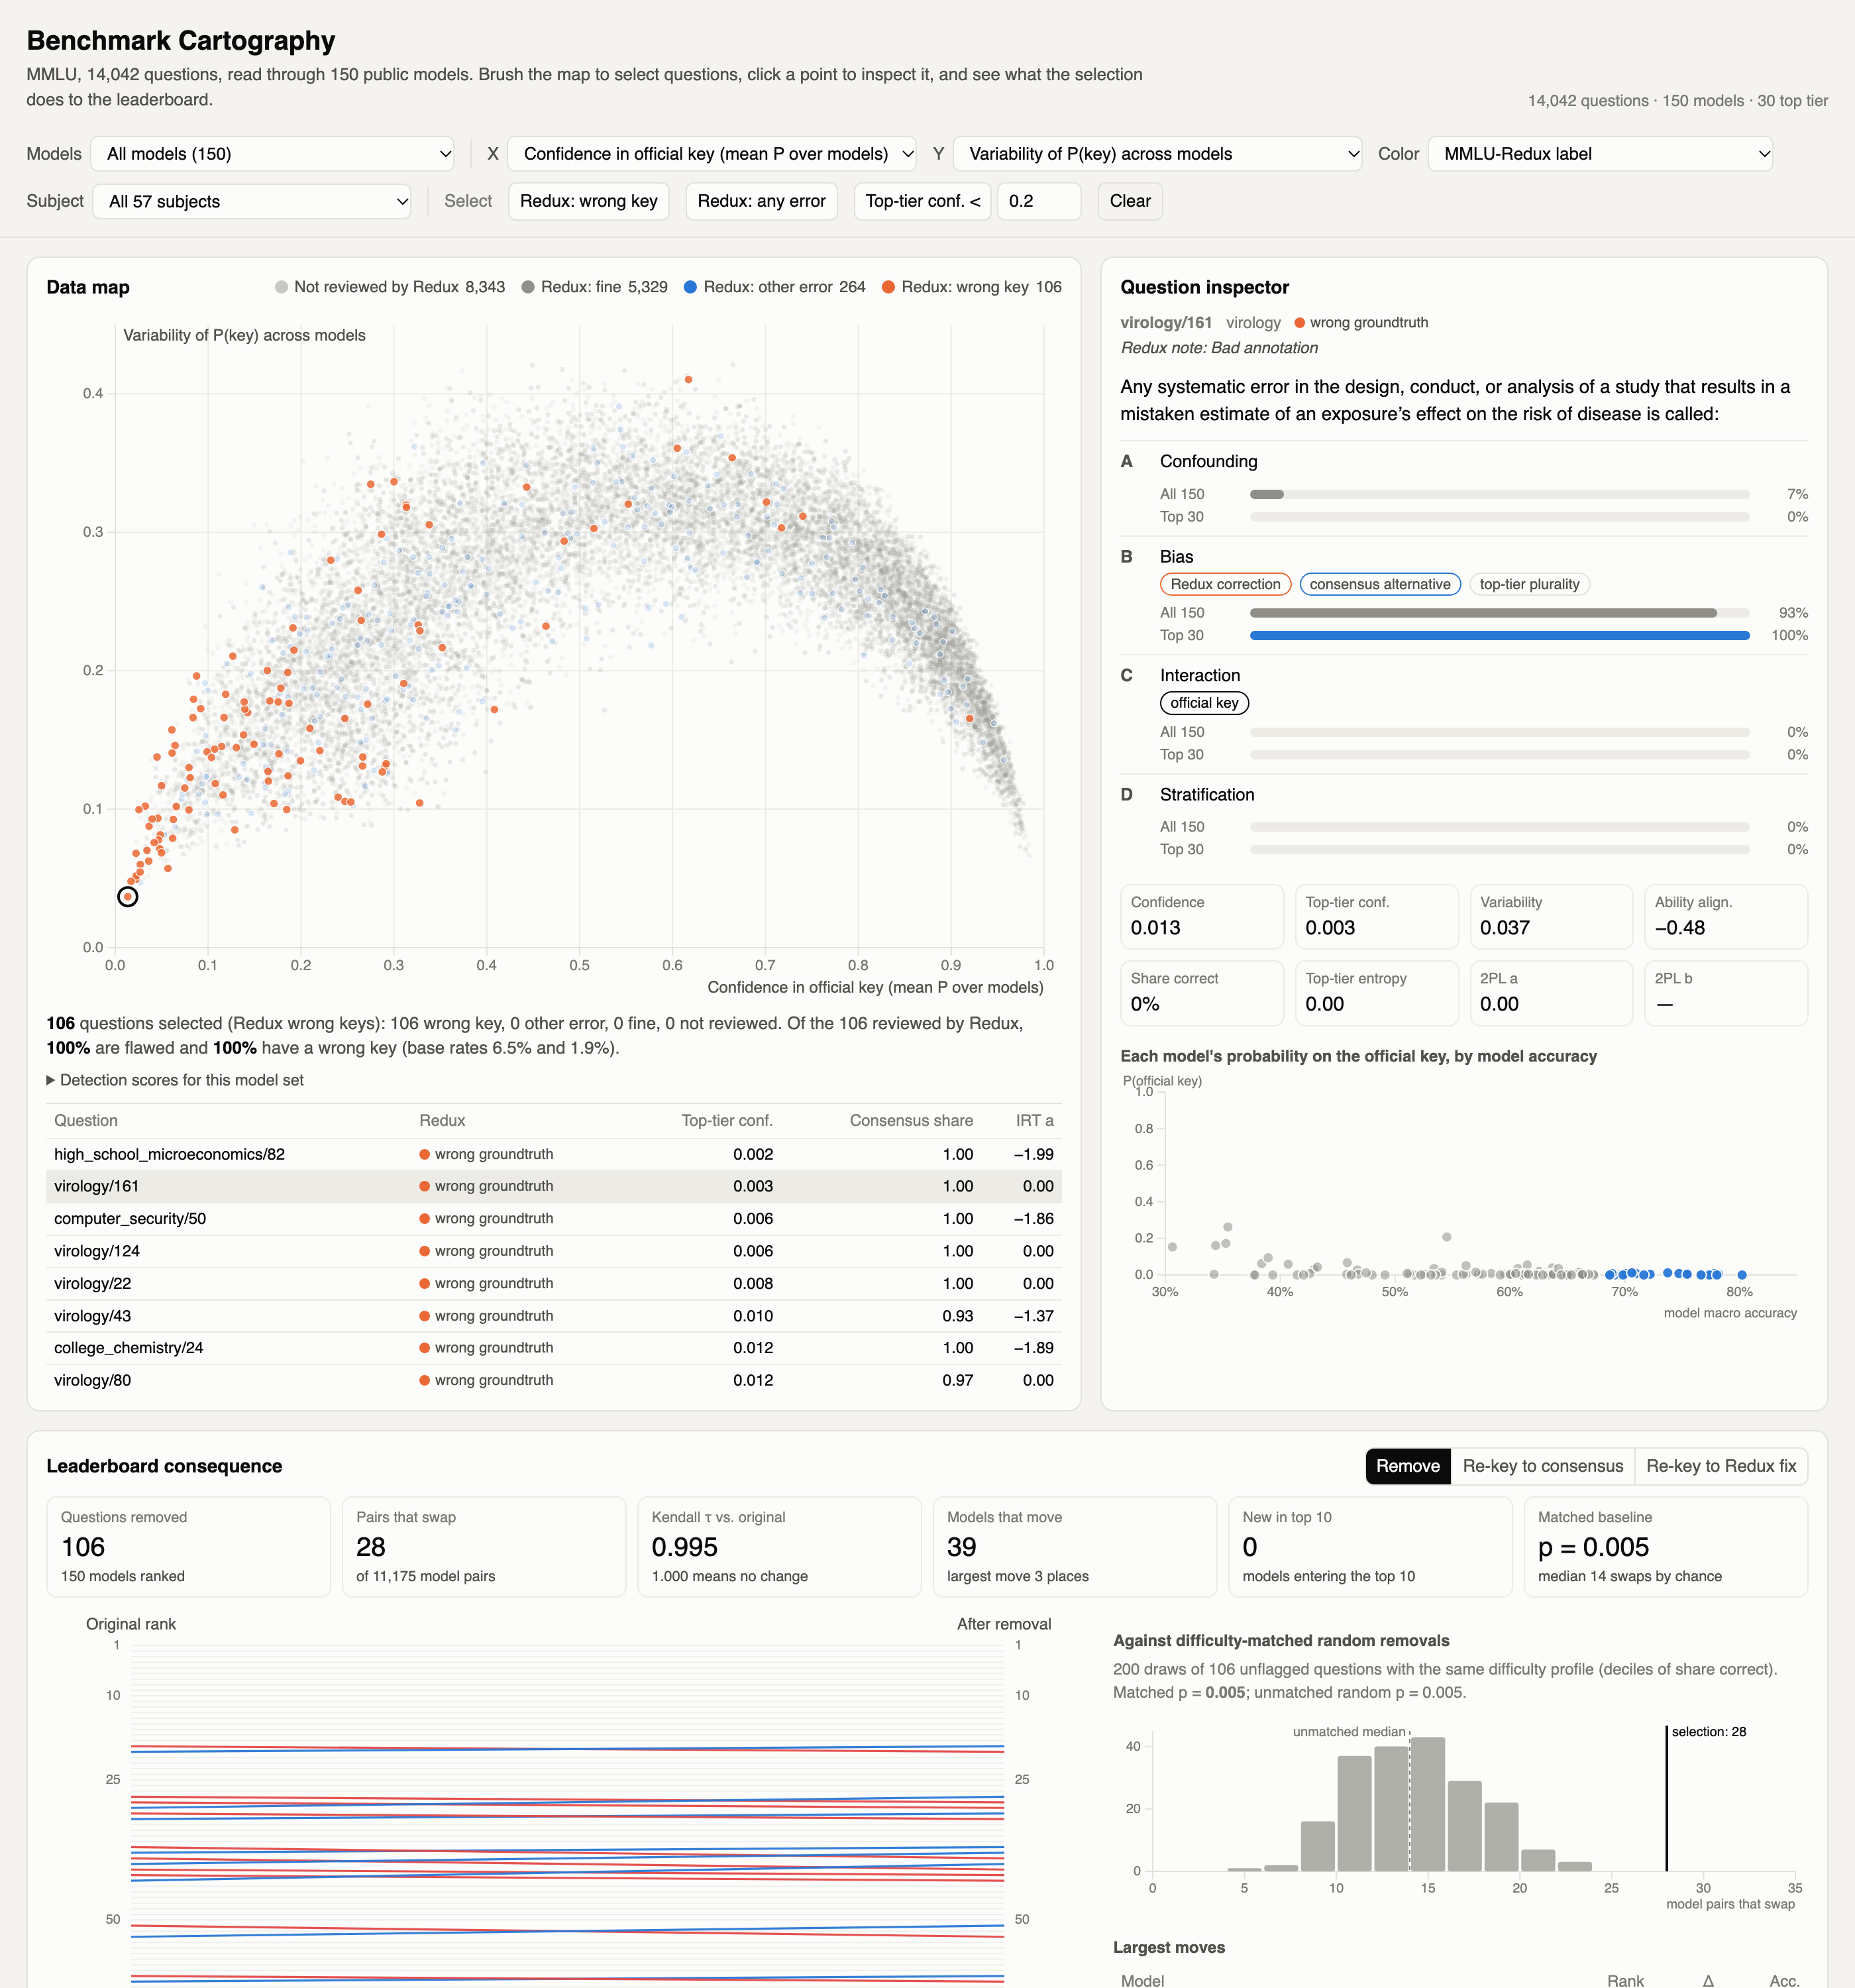
\includegraphics[width=0.86\textwidth]{fig_tool.png}
  \caption{The tool with the 106 MMLU-Redux wrong keys selected. \textbf{Data map} (left): every MMLU
  question by confidence and variability; selected questions are listed below it. \textbf{Question
  inspector} (right): virology/161, where 100\% of the top 30 models choose B, the option MMLU-Redux
  says is correct, and P(key) is near zero for every model regardless of its accuracy.
  \textbf{Leaderboard consequence} (bottom): removing the selection swaps 28 model pairs; the slope
  chart shows who moves, and the histogram compares the swap count with 200 difficulty-matched
  random removals.}
  \label{fig:tool}
\end{figure}

\textbf{Tasks.} We designed for an analyst auditing a benchmark, with three tasks: \emph{T1 locate}
regions of suspicious questions; \emph{T2 judge} a single question (is the key wrong, is the question
ambiguous, or is it just hard?); \emph{T3 weigh consequence} (would fixing these questions change any
conclusion drawn from the leaderboard?). The three core views map one-to-one onto these tasks and are
linked by a single selection (Figure~\ref{fig:tool}).

\textbf{Data map (T1).} All 14,042 questions are drawn on a canvas with an SVG overlay for axes and
brushing, so the full benchmark stays interactive. The axes default to confidence and variability,
as in Dataset Cartography, and can be switched to any score, including the top-tier ones. Color shows
the MMLU-Redux label (gray for the 8,343 unchecked questions, with orange reserved for wrong keys) or a
continuous score such as consensus share. Brushing selects questions (Shift adds), presets select the
Redux wrong keys, all Redux errors, or all questions below a top-tier-confidence threshold, and a
subject filter narrows the map. A collapsible table reports the AUPRC of each score for the current
model set, so the map's encodings can be checked against ground truth.

\textbf{Question inspector (T2).} Clicking a point or table row shows the question and options, and
for each option two bars: the share of all 150 models and of the top 30 that chose it. Tags mark the
official key, the consensus alternative and, where it exists, the Redux correction. Below, eight
score tiles and a strip plot of each model's $p_m(q)$ against its macro accuracy show the
\emph{shape} of the disagreement: a hard but correct question rises to the right; a wrong key is
flat near zero or falls as models get stronger.

\textbf{Leaderboard consequence (T3).} The selection can be removed, re-keyed to the consensus
alternative, or re-keyed to the Redux correction. The tool recomputes every model's macro accuracy in
the browser and reports pair swaps, Kendall's $\tau$, models that move and models entering the top 10;
a slope chart shows each model's rank before and after. To answer ``is this more than chance?'', it
draws 200 random sets with the same difficulty profile (deciles of correctness) from questions outside
the selection that MMLU-Redux did not flag, applies the same action, and shows the distribution of swap
counts with the selection's value and a $p$-value $(1+\#\{\text{draws}\ge\text{observed}\})/(201)$.
An unmatched baseline is shown alongside, so the effect of difficulty alone is visible.

\textbf{Model subsets.} A menu recomputes all scores, the map and the leaderboard for a subset of
models: base (pretrained) models only (53), the strongest model per family (29), two random halves
stratified by family (75 each), or all models except the two whose names mention MMLU. This tests
whether a flag depends on a particular group of models, a risk since many fine-tunes share a base.

\textbf{Study mode.} Adding \texttt{?study} to the URL hides every MMLU-Redux label, color, preset and
correction, so experts judge questions from model evidence alone, and adds a button that selects the
fixed study set (Section~\ref{sec:study}).

\textbf{Implementation.} A Python pipeline writes three static files (question scores as columnar
JSON, model metadata, and an 8-bit matrix of votes and $p_m(q)$ for all model--question pairs, 4\,MB).
The front end is plain D3 v7 with no build step, served from GitHub Pages. Scores recomputed in the
browser match the Python pipeline to within 0.003 (from 8-bit quantisation), and the top tier and
consensus alternatives match exactly. Colors follow a validated palette with separate light and
dark themes.

\section{Results}

\subsection{RQ1: wrong keys occupy a distinct region of the map}

\begin{figure}[!htb]
  \centering
  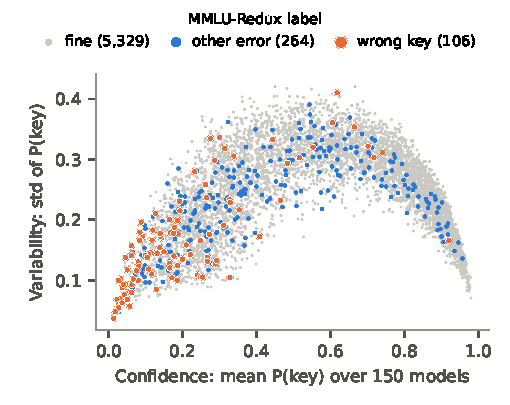
\includegraphics[width=0.49\textwidth]{fig_map.pdf}\hfill
  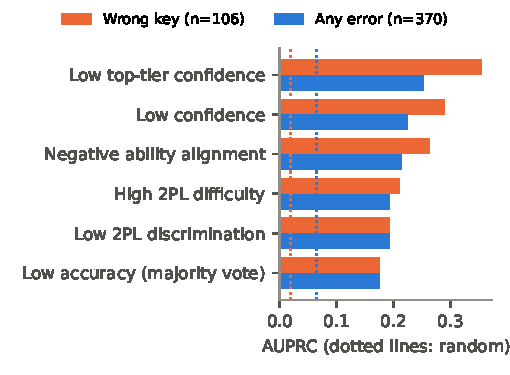
\includegraphics[width=0.49\textwidth]{fig_auprc.pdf}
  \caption{\textbf{Left:} the 5,699 MMLU-Redux questions on the data map. Wrong keys gather in the
  low-confidence, low-variability corner, where nearly every model rejects the key; other errors
  spread through the middle. \textbf{Right:} AUPRC for finding wrong keys and any error, with each
  score oriented so that higher means more suspicious. Dotted lines are the random baselines.}
  \label{fig:map}
\end{figure}

Wrong keys separate clearly from fine questions (Figure~\ref{fig:map}, left). Their median top-tier
confidence is 0.12, against 0.82 for fine questions, and 65\% of them have top-tier confidence
below 0.2, against 6\% of fine questions (AUROC 0.91). They also have low variability (median 0.14
vs.\ 0.26): models agree, but against the key. The other error types do not form a region. Their
median top-tier confidence is 0.47--0.67, and AUROC against fine questions is only 0.58--0.72.
Ambiguity and unclear wording lower confidence a little but do not make models converge on another
answer.

\subsection{RQ2: top-tier confidence finds wrong keys best, and overlaps with IRT}

\begin{table}[!htb]
\centering\small
\caption{AUPRC on the 5,699 MMLU-Redux questions (higher is better). Random equals the base rate.}
\label{tab:auprc}
\begin{tabular}{@{}lcc@{}}
\toprule
Score (higher = more suspicious) & Wrong key ($n=106$) & Any error ($n=370$) \\
\midrule
Random & 0.019 & 0.065 \\
Low accuracy (majority vote against the key) & 0.176 & 0.176 \\
Low 2PL discrimination & 0.192 & 0.192 \\
High 2PL difficulty & 0.211 & 0.193 \\
Negative ability alignment & 0.263 & 0.213 \\
Low confidence & 0.290 & 0.224 \\
\textbf{Low top-tier confidence} & \textbf{0.355} & \textbf{0.252} \\
\bottomrule
\end{tabular}
\end{table}

Low top-tier confidence is the best single score (Table~\ref{tab:auprc}; Figure~\ref{fig:map}, right):
AUPRC 0.355 for wrong keys (95\% bootstrap CI 0.26--0.47), 19 times the base rate, against 0.211 for
the best 2PL parameter and 0.176 for majority vote. Ranked by it, 19 of the first 25 questions
(76\%) and 41 of the first 100 are wrong keys, and the first 200 contain half of all 106. For the
other error types, every score stays close to random (AUPRC at most 0.04 against base rates of
0.4--2.3\%; full table in \texttt{results/report\_numbers.json}). Many-model agreement detects
wrong keys, not unclear or ambiguous questions.

\textbf{What the scores add beyond IRT.} The overlap with IRT is large, as we expected in our update:
top-tier confidence has a Spearman correlation of $-0.92$ with 2PL difficulty, and ability alignment
$0.94$ with 2PL discrimination. To test whether our scores add information, we trained logistic
regressions with 5-fold cross-validation grouped by subject. For wrong keys, 2PL parameters alone
reach AUPRC 0.196, our scores alone 0.248, and both together 0.275; for any error, all three are about
0.19--0.20. So the gain is real but modest, and specific to wrong keys. We do not claim our scores
replace IRT. Their value is in what they let an analyst do next:
\begin{itemize}
  \item \emph{The consensus alternative proposes a fix.} For the 101 wrong keys with a single
    corrected answer, the top tier's preferred alternative is MMLU-Redux's correction in 78\% of cases,
    and in 87\% (62 of 71) when at least half of the top tier agrees. IRT gives a number, not an answer.
  \item \emph{The top tier separates ``hard'' from ``rejected''.} 2PL is fitted on all models' 0/1
    correctness; restricting to the strongest models is what lifts AUPRC from 0.29 (all models) to
    0.36, and the inspector shows both tiers side by side.
  \item \emph{Wrong key vs.\ ambiguous remains hard.} Among low-confidence questions (top-tier
    confidence below 0.3), consensus share separates wrong keys from ambiguous ones only moderately
    (AUROC 0.66; median share 0.87 vs.\ 0.62), no better than 2PL difficulty (0.69). This is why the
    tool shows the evidence to a person rather than a verdict, and it motivates RQ4.
\end{itemize}

\subsection{RQ3: known errors reorder the middle of the leaderboard, not the top}

\begin{table}[!htb]
\centering\small
\caption{Effect on the ranking of 150 models (11,175 pairs). Baselines: 1,000 random sets matched on
difficulty deciles, drawn from questions MMLU-Redux did not flag, with the same action applied.}
\label{tab:rq3}
\begin{tabular}{@{}lccccccc@{}}
\toprule
Action & Qs & Pair swaps & Kendall $\tau$ & Moved & Max move & Matched median & $p$ \\
\midrule
Remove Redux wrong keys & 106 & 28 & 0.995 & 39 & 3 & 14 & 0.001 \\
Remove all Redux-flagged & 370 & 42 & 0.993 & 56 & 3 & 28 & 0.018 \\
Re-key wrong keys to consensus & 106 & 50 & 0.991 & 57 & 5 & 28 & 0.001 \\
Re-key to MMLU-Redux fix & 100 & 44 & 0.992 & 56 & 5 & -- & -- \\
\bottomrule
\end{tabular}
\end{table}

\begin{figure}[!htb]
  \centering
  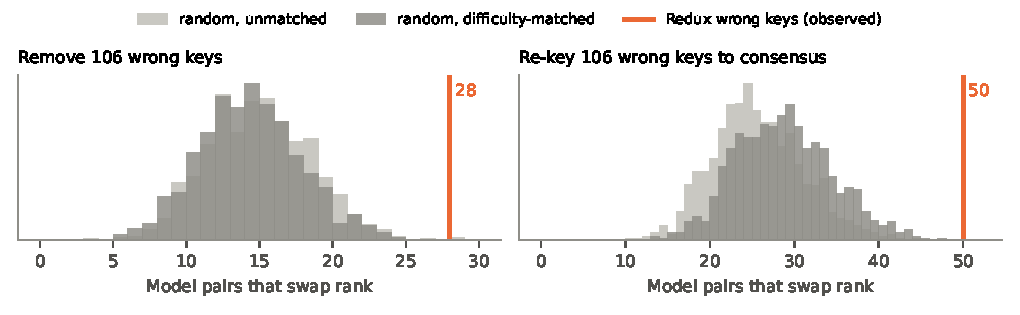
\includegraphics[width=\textwidth]{fig_rq3.pdf}
  \caption{Pair swaps from the 106 wrong keys (orange) against 1,000 random sets of the same size,
  difficulty-matched (dark) and unmatched (light). Left: removal. Right: re-keying to the top tier's
  consensus answer, where each random set is re-keyed to its own consensus alternative.}
  \label{fig:rq3}
\end{figure}

Removing the 106 wrong keys swaps 28 model pairs, twice the median of difficulty-matched random
removals (14; $p=0.001$, Table~\ref{tab:rq3}, Figure~\ref{fig:rq3}). Correcting them instead of
removing them has a larger effect: re-keying to the consensus answer swaps 50 pairs against a matched
median of 28, and re-keying to the MMLU-Redux correction swaps 44, moving 56 of 150 models by up to 5
places. Removing all 370 Redux-flagged questions also reorders more than chance (42 vs.\ 28, $p=0.018$).
The matched and unmatched baselines have similar medians here, so difficulty alone does not explain
the effect.

The effect is real but small: Kendall's $\tau$ stays above 0.99, no model enters or leaves the top
10, and the moves happen in the crowded middle of the ranking, where neighbouring models are a
fraction of a point apart. Our reading is that MMLU's known errors do not change which models lead,
but they do change comparisons between similar models, which is how leaderboards are often used
(``our fine-tune beats the base model''). A small effect was a possible outcome we named in the
proposal, and it is useful to report.

One contrast is worth noting. Removing the 370 questions \emph{our} score ranks most suspicious
swaps only 21 pairs, fewer than equally hard random questions (matched mean 35; computed by
\texttt{analysis/02\_ranking.py}). Questions the top tier rejects tend to be missed by every model,
so they separate models less than ordinary hard questions do. \fillin{Arman: confirm this
interpretation or replace it.}

\subsection{Robustness to the choice of models}

\begin{table}[!htb]
\centering\small
\caption{Recomputing everything on model subsets (from the tool; 200 matched draws). AUPRC is for
low top-tier confidence on wrong keys; swaps are for removing the 106 wrong keys.}
\label{tab:robust}
\begin{tabular}{@{}lcccc@{}}
\toprule
Model set & Models & AUPRC (wrong key) & Pair swaps & Matched median \\
\midrule
All models & 150 & 0.356 & 28 & 14 \\
Base (pretrained) models only & 53 & 0.317 & 5 & 1 \\
Strongest model per family & 29 & 0.374 & 0 & 0 \\
Random half A (stratified by family) & 75 & 0.367 & 8 & 3 \\
Random half B & 75 & 0.314 & 5 & 2 \\
Without the 2 models whose names mention MMLU & 148 & 0.357 & -- & -- \\
\bottomrule
\end{tabular}
\end{table}

Detection is stable across model sets (AUPRC 0.31--0.37, Table~\ref{tab:robust}). Fine-tunes that
share a base model do not drive the result: keeping only the strongest model per family gives the
highest AUPRC. The ranking effect shrinks with fewer models, as expected, since there are fewer pairs
and wider gaps between them. With one model per family no pair swaps, so the reordering in the full
leaderboard happens among closely related models. Excluding the two models trained on MMLU-named data
changes nothing. \fillin{HELM cross-check: not done; say so or drop.}

\subsection{Likely errors outside MMLU-Redux}

Of the 8,343 questions MMLU-Redux did not review, 630 have top-tier confidence below 0.2, and 289 of
those also have at least 80\% of the top tier agreeing on one alternative (listed in
\texttt{results/candidates\_outside\_redux.csv}). Precision among Redux-checked questions suggests
many of these are wrong keys, but we have hand-checked only a few. Two examples from our study set,
\fillin{pending confirmation by both authors}: \emph{miscellaneous/468} asks which actress played the
Vulcan Saavik in \emph{Star Trek II}; the key says Helen Hunt, while 83\% of the top tier choose Kirstie
Alley, who played the role. \emph{high\_school\_psychology/53} asks which is \emph{not} a primary facial
expression; the key says surprise, which is one of the basic expressions, and 97\% of the top tier
choose love. \fillin{optional: hand-check the top 20 candidates and report how many are wrong keys.}

\section{Expert Study (RQ4)}
\label{sec:study}

Following the proposal feedback, this is a formative, qualitative study: no control condition, no
timing and no statistical claims.

\textbf{Participants.} \fillin{n} people who work on LLM evaluation, NLP benchmarks or data quality
\fillin{roles and years of experience, e.g. ``3 PhD students, 1 research engineer''}. We recorded
role and experience only.

\textbf{Procedure.} Each 30--45 minute session over video call used the tool in study mode, with no
MMLU-Redux labels visible. One of us facilitated from a fixed script and the other took notes. After a
scripted 5-minute tour, participants (1) triaged a fixed set of 8 questions, saying for each whether
the key is wrong, the question is ambiguous, or it is hard and the key is right, with confidence 1--5
and the evidence that convinced them; (2) used the leaderboard view to decide whether the questions they
judged broken would change how they report MMLU, including re-keying and switching model subsets;
and (3) answered debrief questions. The 8 questions all have low top-tier confidence, so the scores
alone cannot separate them: 4 wrong keys (2 from MMLU-Redux, 2 candidates outside it), 1 ambiguous,
and 3 hard questions whose key is correct, including one where 77\% of the top tier agree on a wrong
alternative. Both of us coded the notes independently and merged the codes.

\textbf{Results.} \fillin{Verdict table: per question, participants' verdicts vs. the reference.}

\fillin{3--4 themes, each with 1--2 short quotes. Candidates to look for: which evidence was decisive
(top-tier bars vs. all-model bars vs. the strip plot vs. scores); over-trust of model consensus on the
hard-but-correct questions; how participants read the matched baseline and p-value; whether the subset
toggle changed their conclusions; what they would add.}

\fillin{Usability problems found, and which we fixed.}

\section{Discussion and Limitations}

\textbf{Agreement is evidence, not proof.} Strong models share training data and can share a
misconception, so consensus against the key can be wrong; our study set includes such a case on
purpose. We call flags \emph{likely} errors, and the tool shows the evidence behind them rather than
a verdict.

\textbf{What the map is for.} A sorted table of top-tier confidence would find the same wrong keys.
The map's role is overview and triage: it shows that wrong keys sit in one corner while other errors
do not, lets an analyst brush a region rather than pick a threshold, and connects to the inspector and
the leaderboard view, which a table does not. \fillin{Add what participants said about map vs. table.}

\textbf{Limitations.} One benchmark and one harness version; 5-shot log-likelihood scoring rather than
generation; 150 models from one leaderboard, which over-represents 7B fine-tunes of a few bases; ground
truth from one re-annotation effort, which itself has disagreements; only wrong keys are detectable,
not ambiguous questions; and a small expert study with colleagues rather than a sample of
practitioners. The tool's numbers use 8-bit probabilities and 200 random draws, while the tables use
the full-precision data and 1,000.

\section{Conclusion}

Reading a benchmark through 150 models turns Dataset Cartography into an audit tool for evaluation
data. Low confidence among the strongest models finds MMLU's wrong keys far better than chance and
better than 2PL IRT, and their consensus usually names the right answer. Fixing the known wrong keys
reorders the leaderboard more than chance, but only among closely matched models, not at the top.
Linking these findings in one interactive tool lets an analyst move from a suspicious region, to the
evidence for one question, to its consequence for the ranking, and \fillin{one sentence on what the
expert study showed}.

\textbf{Team contributions.} Padmapriya Venkatesh built the data pipeline, scores and 2PL fit (Stage 1)
and the D3 tool (Stage 3). Arman Samayam led the detection and ranking analyses (Stage 2). Both
designed and ran the expert study and wrote the report.

\textbf{Reproducibility.} Code, cached data with checksums, and all scripts are at
\url{https://github.com/ArmanSam17/Benchmark-Cartography}. \texttt{analysis/01\_detection.py} and
\texttt{analysis/02\_ranking.py} produce the RQ2 and RQ3 tables; \texttt{report/report\_numbers.py}
produces the remaining numbers and figures.

\small
\begin{thebibliography}{99}\setlength{\itemsep}{1pt}
\bibitem{cartography} S. Swayamdipta, R. Schwartz, N. Lourie, Y. Wang, H. Hajishirzi, N. A. Smith, Y. Choi.
  Dataset Cartography: Mapping and Diagnosing Datasets with Training Dynamics. EMNLP 2020.
\bibitem{pervasive} C. G. Northcutt, A. Athalye, J. Mueller. Pervasive Label Errors in Test Sets
  Destabilize Machine Learning Benchmarks. NeurIPS Datasets and Benchmarks 2021.
\bibitem{cl} C. G. Northcutt, L. Jiang, I. L. Chuang. Confident Learning: Estimating Uncertainty in
  Dataset Labels. JAIR 2021.
\bibitem{rodriguez} P. Rodriguez, J. Barrow, A. M. Hoyle, J. P. Lalor, R. Jia, J. Boyd-Graber.
  Evaluation Examples Are Not Equally Informative: How Should That Change NLP Leaderboards? ACL 2021.
\bibitem{tiny} F. M. Polo, L. Weber, L. Choshen, Y. Sun, G. Xu, M. Yurochkin. tinyBenchmarks:
  Evaluating LLMs with Fewer Examples. ICML 2024.
\bibitem{redux} A. P. Gema et al. Are We Done with MMLU? NAACL 2025.
\bibitem{calibrate} P. Xenopoulos, J. Rulff, L. G. Nonato, B. Barr, C. Silva. Calibrate: Interactive
  Analysis of Probabilistic Model Output. IEEE VIS 2022.
\bibitem{zeno} \'A. A. Cabrera, E. Fu, D. Bertucci, K. Holstein, A. Talwalkar, J. I. Hong, A. Perer.
  Zeno: An Interactive Framework for Behavioral Evaluation of Machine Learning. CHI 2023.
\bibitem{helm} P. Liang et al. Holistic Evaluation of Language Models. TMLR 2023.
\bibitem{openllm} Hugging Face. Open LLM Leaderboard (archived), per-model evaluation details.
  Accessed Oct 2026.
\bibitem{mmlu} D. Hendrycks, C. Burns, S. Basart, A. Zou, M. Mazeika, D. Song, J. Steinhardt.
  Measuring Massive Multitask Language Understanding. ICLR 2021.
\end{thebibliography}

\end{document}
